 \documentclass[11pt]{beamer}
\usetheme{Warsaw}
\usepackage[utf8]{inputenc}
\usepackage{amsmath}
\usepackage{array}
\usepackage{amsfonts}
\usepackage{amssymb}
\usepackage{tikz}
\usetikzlibrary{arrows,automata}
%\usepackage[latin1]{inputenc}

\author{Team Expeditus}
\title{UAV Autonomous Landing}
%\setbeamercovered{transparent} 
%\setbeamertemplate{navigation symbols}{} 
%\logo{} 
\institute{SDSMT MCS} 
%\date{} 
%\subject{} 
\begin{document}

\begin{frame}
\titlepage
\end{frame}

%\begin{frame}
%\tableofcontents	
%\end{frame}

\begin{frame}{Introduction}
\textbf{UAV Autonomous Landing Project}\\
\vspace{12mm}
\textbf{Team Expeditus}\\
Jonathan Dixon, Dylan Geyer, Christopher Smith, Steven Huerta\\ 
\vspace{6mm}
\textbf{Sponsor}\\
Dr. Larry Pyeatt\\
\end{frame}


\begin{frame}{Goal}
Demonstrate the capability of a UAV to autonomously take-off, navigate through some waypoints, return to the landing pad, and land with a minimum of distance and orientation error. 
\end{frame}


\begin{frame}{Requirements}
\textbf{Goal}\\
\begin{itemize}
\item receive a set of waypoints
\item autonomously take-off
\item navigate through waypoints
\item return to launch pad
\item \textbf{land with $\pm$.1m distance and $\pm$15$^{\circ}$ orientation error}
\end{itemize}
\vspace{6mm}
\textbf{Limitations}\\
\begin{itemize}
\item landing platform is a fixed position
\item landing platform is a stable, horizontal surface
\item environment is ideal(no wind, gps available, no obstacles)
\end{itemize}
\end{frame}


\begin{frame}{User Stories/Backlog}

\begin{itemize}
\item \textbf{User 1(U-1):}\\ As a user, I want to communicate the waypoints to the UAV.
\item \textbf{Owner 1(O-1):}\\ As an owner, I want the UAV to autonomously take-off from the landing pad.
\item \textbf{Owner 2(O-2):}\\ As an owner, I want the UAV to autonomously navigate through a set of waypoints.
\item \textbf{Owner 3(O-3):}\\ As an owner, I want the UAV to autonomously return to the location of the landing pad.
\item \textbf{Owner 4(O-4):}\\ As an owner, I want the UAV to autonomously land on the landing pad without damaging the craft.
\item \textbf{Owner 5(O-5):}\\ As an owner, I want the UAV to autonomously land on the landing pad with the correct orientation.
\item \textbf{Common:}\\ Tasks relating to more than one user story(i.e. resolving dependencies).
\end{itemize}

\end{frame}

\begin{frame}{U-1}
\textbf{As a user, I want to communicate the waypoints to the UAV.}
\begin{tabular}{| c | >{\raggedright}m{4cm} | c | c |}\hline
Task No. & Task & Date Completed & Sprint\\\hline
1 & Review previous method/interface for communicating coordinates to UAV. & 10/05/15 & 1 \\\hline
2 & Review code that communicates with quadrotor & 10/16/15 & 2 \\\hline
3 & Review code that allows a user to input waypoints & 10/16/15 & 2\\\hline
4 & Modify/Rewrite imlementation as necessary & 01/23/2016 & 4\\\hline

\end{tabular}
\end{frame}


\begin{frame}{O-1}
\textbf{As an owner, I want the UAV to autonomously take-off from the landing pad.}
\begin{tabular}{| c | >{\raggedright}m{4cm} | c | c |}\hline
Task No. & Task & Date Completed & Sprint\\\hline
1 & Review previous implementation for autonomous take-off. & 10/05/15 & 1 \\\hline
2 & Review code that enables the quadrotor to autonomously take-off from landing pad & 10/16/15 & 2 \\\hline
3 & Modify/Rewrite take-off imlementation as necessary & 01/23/2016 & 4 \\\hline
\end{tabular}
\end{frame}


\begin{frame}{O-2}
\textbf{As an owner, I want the UAV to autonomously navigate through a set of waypoints.}
\begin{tabular}{| c | >{\raggedright}m{4cm} | c | c |}\hline
Task No. & Task & Date Completed & Sprint\\\hline
1 & Review previous implementation for navigating waypoints. & 10/05/15 & 1 \\\hline
2 & Review code that enables the quadrotor to autonomously navigate through a series of way-points & 10/16/15 & 2 \\\hline
3 & Modify/Rewrite take-off imlementation as necessary & 01/23/2016 & 4 \\\hline
\end{tabular}
\end{frame}


\begin{frame}{O-3}
\textbf{As an owner, I want the UAV to autonomously return to the location of the landing pad.}
\begin{tabular}{| c | >{\raggedright}m{4cm} | c | c |}\hline
Task No. & Task & Date Completed & Sprint\\\hline
1 & Review previous implementation to autonomously return to location of landing pad & 10/05/15 & 1 \\\hline
2 & Review code that allows the autonomous return of the UAV to the landing pad. & 10/16/15 & 2 \\\hline
3 & Modify/Rewrite take-off imlementation as necessary & 01/23/2016 & 4 \\\hline
\end{tabular}
\end{frame}


\begin{frame}{O-4}
\textbf{As an owner, I want the UAV to autonomously land on the landing pad without damaging the craft}
\begin{tabular}{| c | >{\raggedright}m{4cm} | c | c |}\hline
Task No. & Task & Date Completed & Sprint\\\hline
1 & Review previous implementation for autonomous landing & 10/05/15 & 1 \\\hline
2 & Install previous implementation & 10/19/15 & 2 \\\hline
3 & Test previous implementation & 10/26/15 & 2\\\hline
\end{tabular}
\end{frame}


\begin{frame}{O-5}
\textbf{As an owner, I want the UAV to autonomously land on the landing pad with the correct orientation.}
\begin{tabular}{| c | >{\raggedright}m{4cm} | c | c |}\hline
Task No. & Task & Date Completed & Sprint\\\hline
1 & Review previous implementation for autonomous landing & 10/05/15 & 1 \\\hline
2 & Install previous implementation & 10/19/15 & 2 \\\hline
3 & Test previous implementation & 10/26/15 & 2\\\hline
\end{tabular}
\end{frame}


\begin{frame}{C}
\textbf{Initial Common Tasks}
\begin{tabular}{| c | >{\raggedright}m{4cm} | c | c |}\hline
Task No. & Task & Date Completed & Sprint\\\hline
1 & Install Ubuntu 14.04 or some other ROS Indigo/Jade distro compliant OS. & 09/25/15 & 1 \\\hline
2 & Setup Gazebo 6.+ & 09/25/15 & 1 \\\hline
3 & Download Rviz package & 09/25/15 & 1\\\hline
4 & Setup Simulation Environment & 11/02/15 & 2 \\\hline
\end{tabular}
\end{frame}


\begin{frame}{C Continued}
\textbf{Initial Common Tasks}
\begin{tabular}{| c | >{\raggedright}m{4cm} | c | c |}\hline
Task No. & Task & Date Completed & Sprint\\\hline
5 & Review previous iteration of project documentation & 09/25/15 & 1 \\\hline
6 & Inspect current quadrotor configuration & 09/28/2015 & 2\\\hline
7 & Identify parts needed for quadrotor & 11/02/2015 & 2 \\\hline
8 & Acquire parts needed for hexrotor & 12/01/2015 & 3 \\\hline
9 & Build UAV & 01/17/16 & 4 \\\hline
10 & Test flight under manual control & 01/17/16 & 4 \\\hline
\end{tabular}
\end{frame}


 \begin{frame}{Sprint 1}
	\large{\textbf{Sprint 1 - Successes}}
\begin{itemize}
	\item Revised project scope
	\item Product Backlog - User Stories
	\item Setup Development Environment
	\item Review previous years hardware and software
\end{itemize}

	\large{\textbf{Sprint 1 - Setbacks}}
	\begin{itemize}
		\item Previous years UAV unusable
		\item Previous years flight code unusable
	\end{itemize}
 \end{frame}
 
 
 \begin{frame}{Sprint 2}
	\large{\textbf{Sprint 2 - Successes}}
	\begin{itemize}
		\item Visual Homography Code repurposed
		\item Created simulation environment
		\item Ordered parts for new Hex-copter
	\end{itemize}
	\large{\textbf{Sprint 2 - Setbacks}}
	\begin{itemize}
		\item Simulation only supports manual control
	\end{itemize}
 \end{frame}
 
 
 \begin{frame}{Sprint 3}
	\large{\textbf{Sprint 3 - Successes}}
	\begin{itemize}
		\item Assembled Frame, Motors, ESC's
		\item Many SITL simulations
		\item Waypoint Publisher publishes mavros commands
		\item Working image homography code
		\item Becoming familiar with python openCV libraries
	\end{itemize}
	\large{\textbf{Sprint 3 - Setbacks}}
	\begin{itemize}
		\item Pixhawk delayed 2 weeks, build not completed
		\item SITL simulations rejected waypoint files
		\item SITL simulations rejected mavros commands
	\end{itemize}
 \end{frame}
 
 
  \begin{frame}{Sprint 3.5 + 4}
  	\large{\textbf{Sprint 3.5 + 4 Successes}}
  	\begin{itemize}
  		\item Finished construction of UAV
  		\item Manual flight of the UAV achieved
  		\item Autonomous flight of the UAV achieved
  		\item GPS Waypoint navigation achieved
  	\end{itemize}
  	\large{\textbf{Sprint 3.5 + 4 Setbacks}}
  	\begin{itemize}
  		\item AR Track Alvar not working
  		\item Simulation tasks abandoned
  	\end{itemize}
  \end{frame}
  
   \begin{frame}{Sprint 5}
   	\large{\textbf{Sprint 5 Successes}}
   	\begin{itemize}
   		\item Non-ROS Alvar reading pose and position
   		\item AR Track Alvar reading pose and position
   		\item Basic off-board control on the Pixhawk
   	\end{itemize}
   	\large{\textbf{Sprint 5 Setbacks}}
   	\begin{itemize}
   		\item Localization in off-board control
   	\end{itemize}
   \end{frame}

%%% End SECTION 1 


%% Begin SECTION 2 
\begin{frame}{Design}
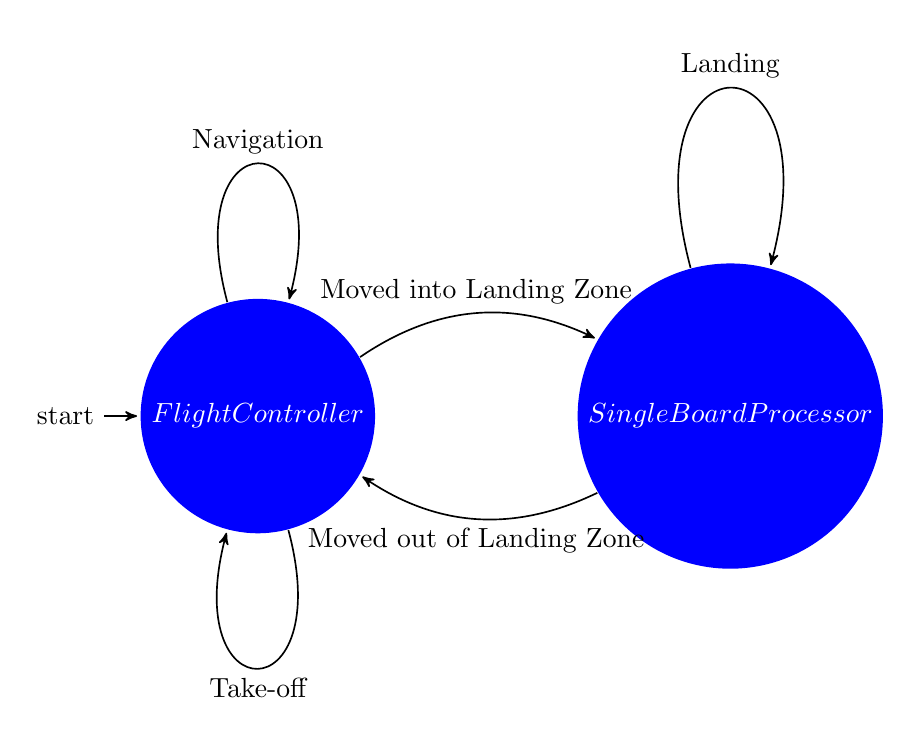
\begin{tikzpicture}[->,>=stealth',shorten >=1pt,auto,node distance=6cm,
                    semithick]
  \tikzstyle{every state}=[fill=blue,draw=none,text=white]

  \node[initial,state] (A)              {$Flight Controller$};
  \node[state]         (B) [right of=A] {$Single Board Processor$};

  \path (A) edge [loop below] node {Take-off} (A)
            edge [loop above]  node {Navigation} (A)
            edge [anchor=center,bend left,above] node {Moved into Landing Zone} (B)
        (B) edge [loop above] node {Landing} (B)
            edge [anchor=center,bend left,left,below]  node {Moved out of Landing Zone} (A);
\end{tikzpicture}
\end{frame}

\begin{frame}{Architecture}
\begin{figure}
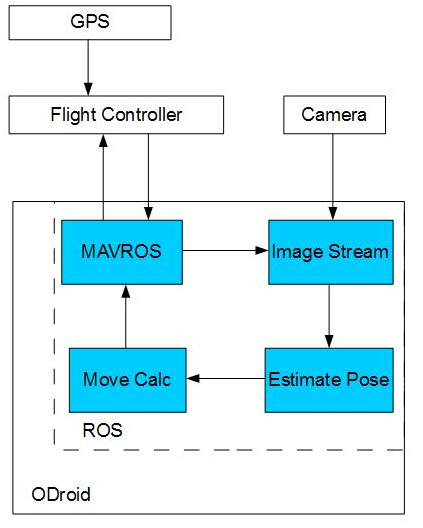
\includegraphics[width=.5\textwidth]{images/broad_approach1}
\end{figure}

\end{frame}

\begin{frame}{Hardware Requirements}
\begin{itemize}
\item ODroid XU4
\item Pixhawk Flight Controller
\item GPS peripheral
\item Camera
\item Battery
\item UAV(Frame, Motors, ESCs, Power Distribution Board)
\end{itemize}

\end{frame}

\begin{frame}{Software Requirements}
\begin{itemize}
\item Mavlink
\item Python
\item OpenCV
\item Robot Operating System(ROS) Indigo/Jade Distro
\item Ubuntu 14.04
\end{itemize}

\end{frame}



% Include Architecture/Design/Tech Specs/& Tools ---Likely will take a few slides 
\begin{frame}{UAV Design \& Tech Specs}
	Physical design of the hex-copter is the \textbf{Turnigy Talon Hexcopter}
	
	\begin{figure}
		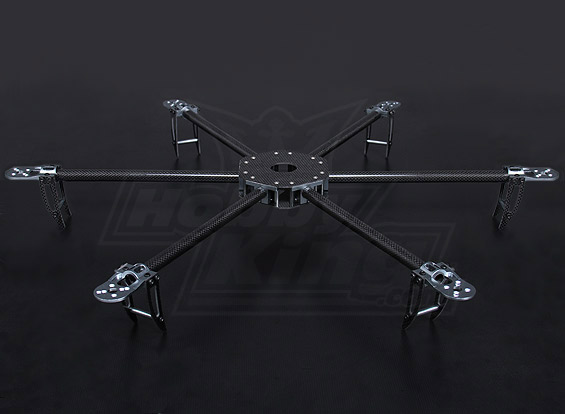
\includegraphics[width=4in]{images/TalonV1.jpg}
	\end{figure}

\end{frame}

% Include Architecture/Design/Tech Specs/& Tools ---Likely will take a few slides 
\begin{frame}{Localization Software Architecture}
	Architecture for communication between ROS nodes for evaluating a local position: \\
	\centering
	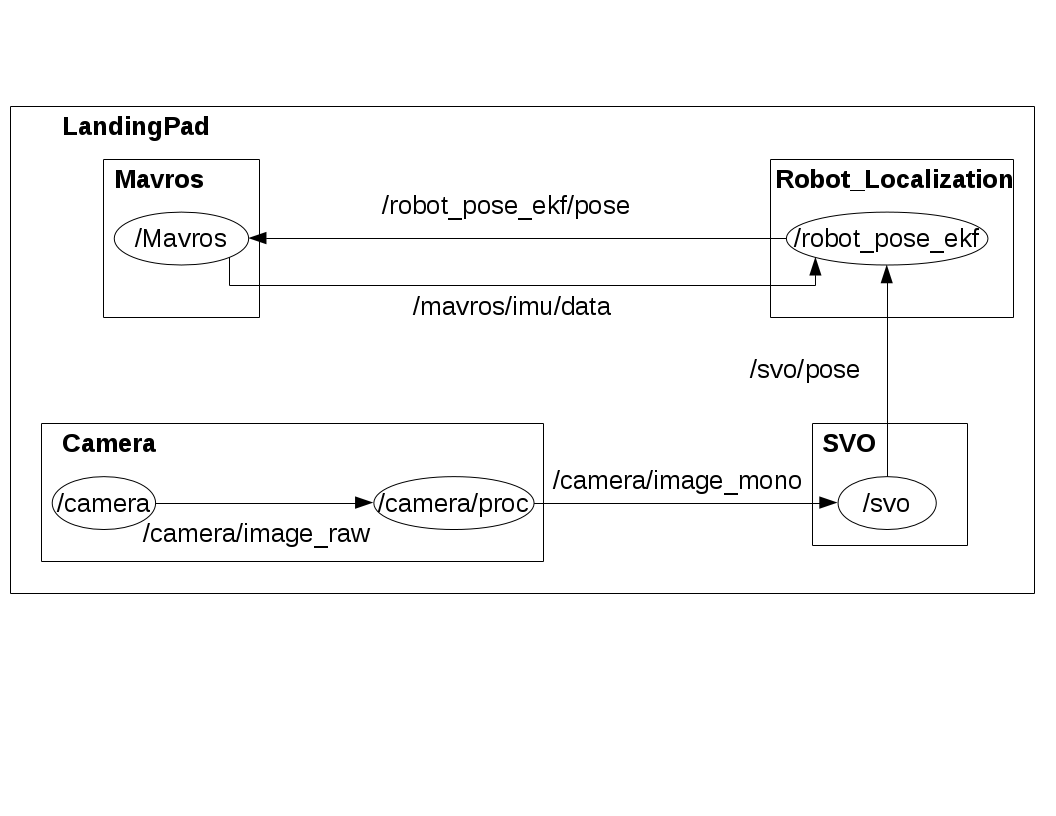
\includegraphics[width=.9\textwidth]{images/localization.png}
\end{frame}

\begin{frame}{Navigation Software Architecture}
	Architecture for communication between ROS nodes to accomplish laninding on the landing pad: \\
	\centering
	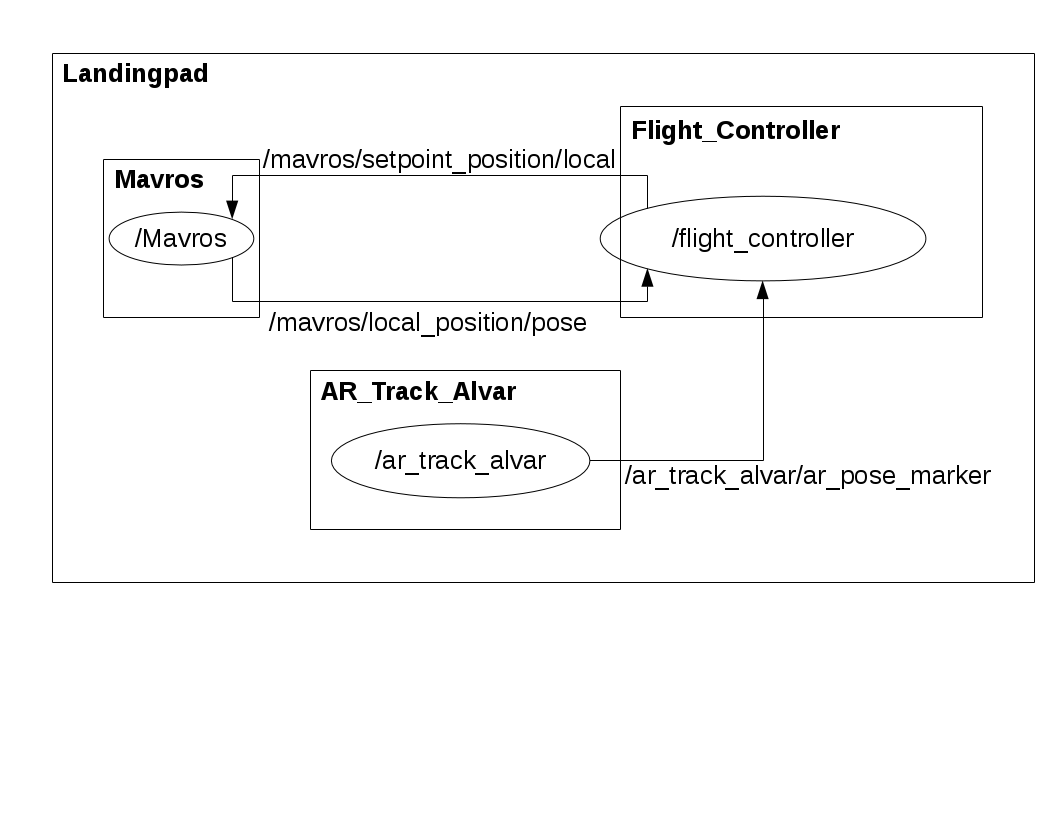
\includegraphics[width=.9\textwidth]{images/navigation.png}
\end{frame}

\begin{frame}{AR Track Alvar Framework}
	AR Track Alvar can provide pose and orientation of the AR tag relative to the frame of the camera: \\
	\centering
	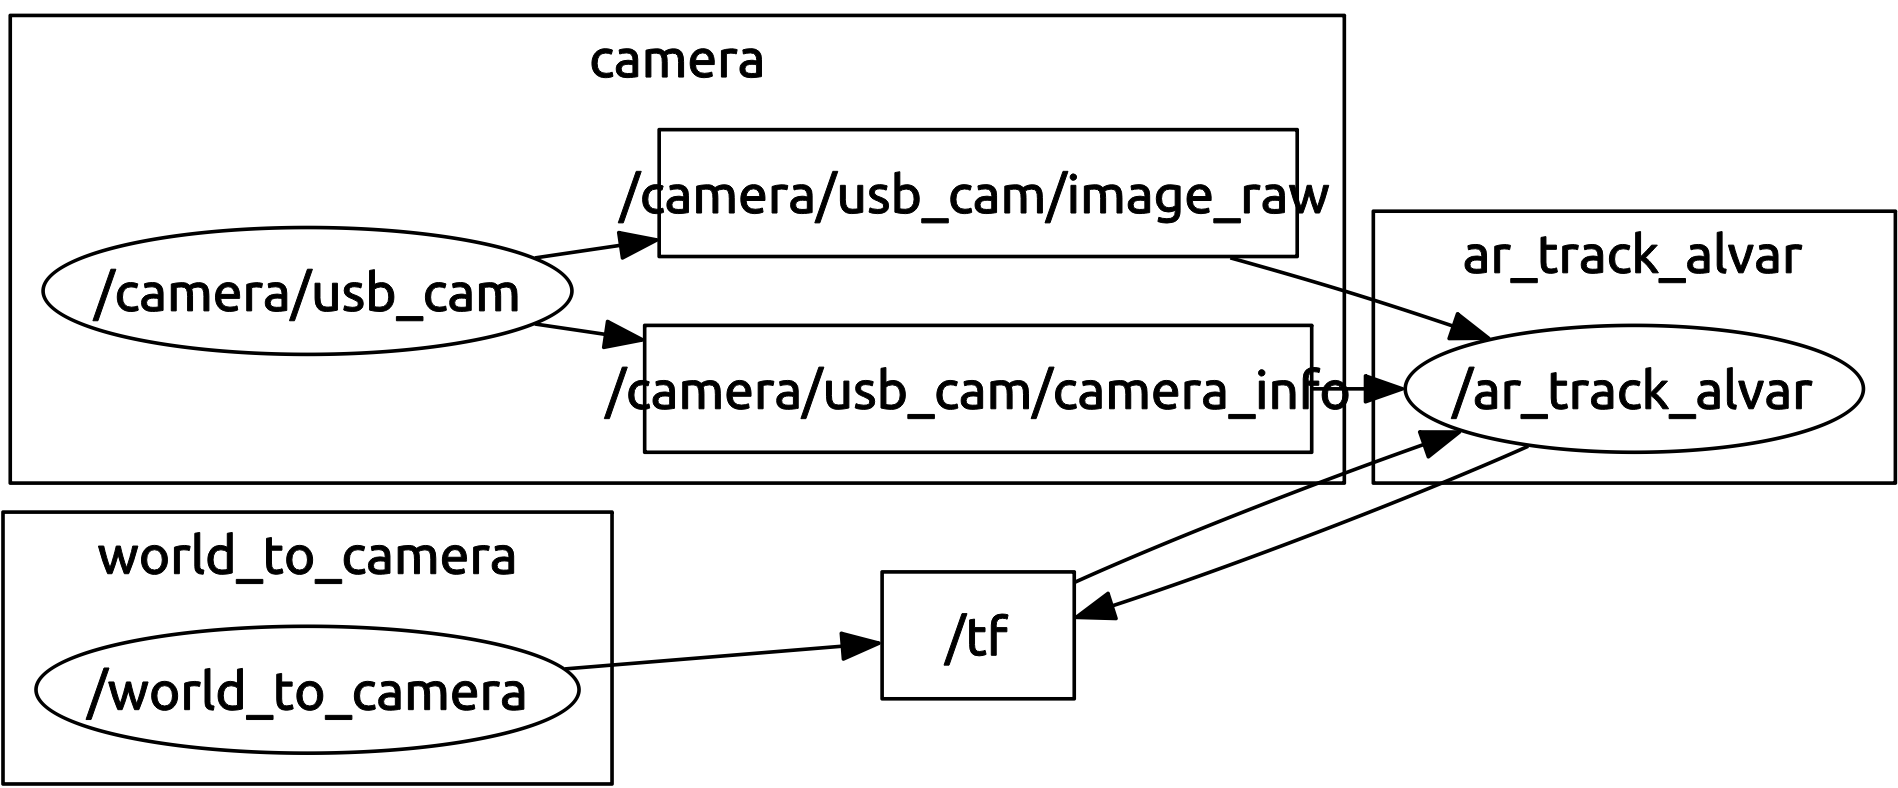
\includegraphics[width=1\textwidth]{images/artrackgraph.png}
\end{frame}

\begin{frame}{AR Track Alvar}
	\centering
	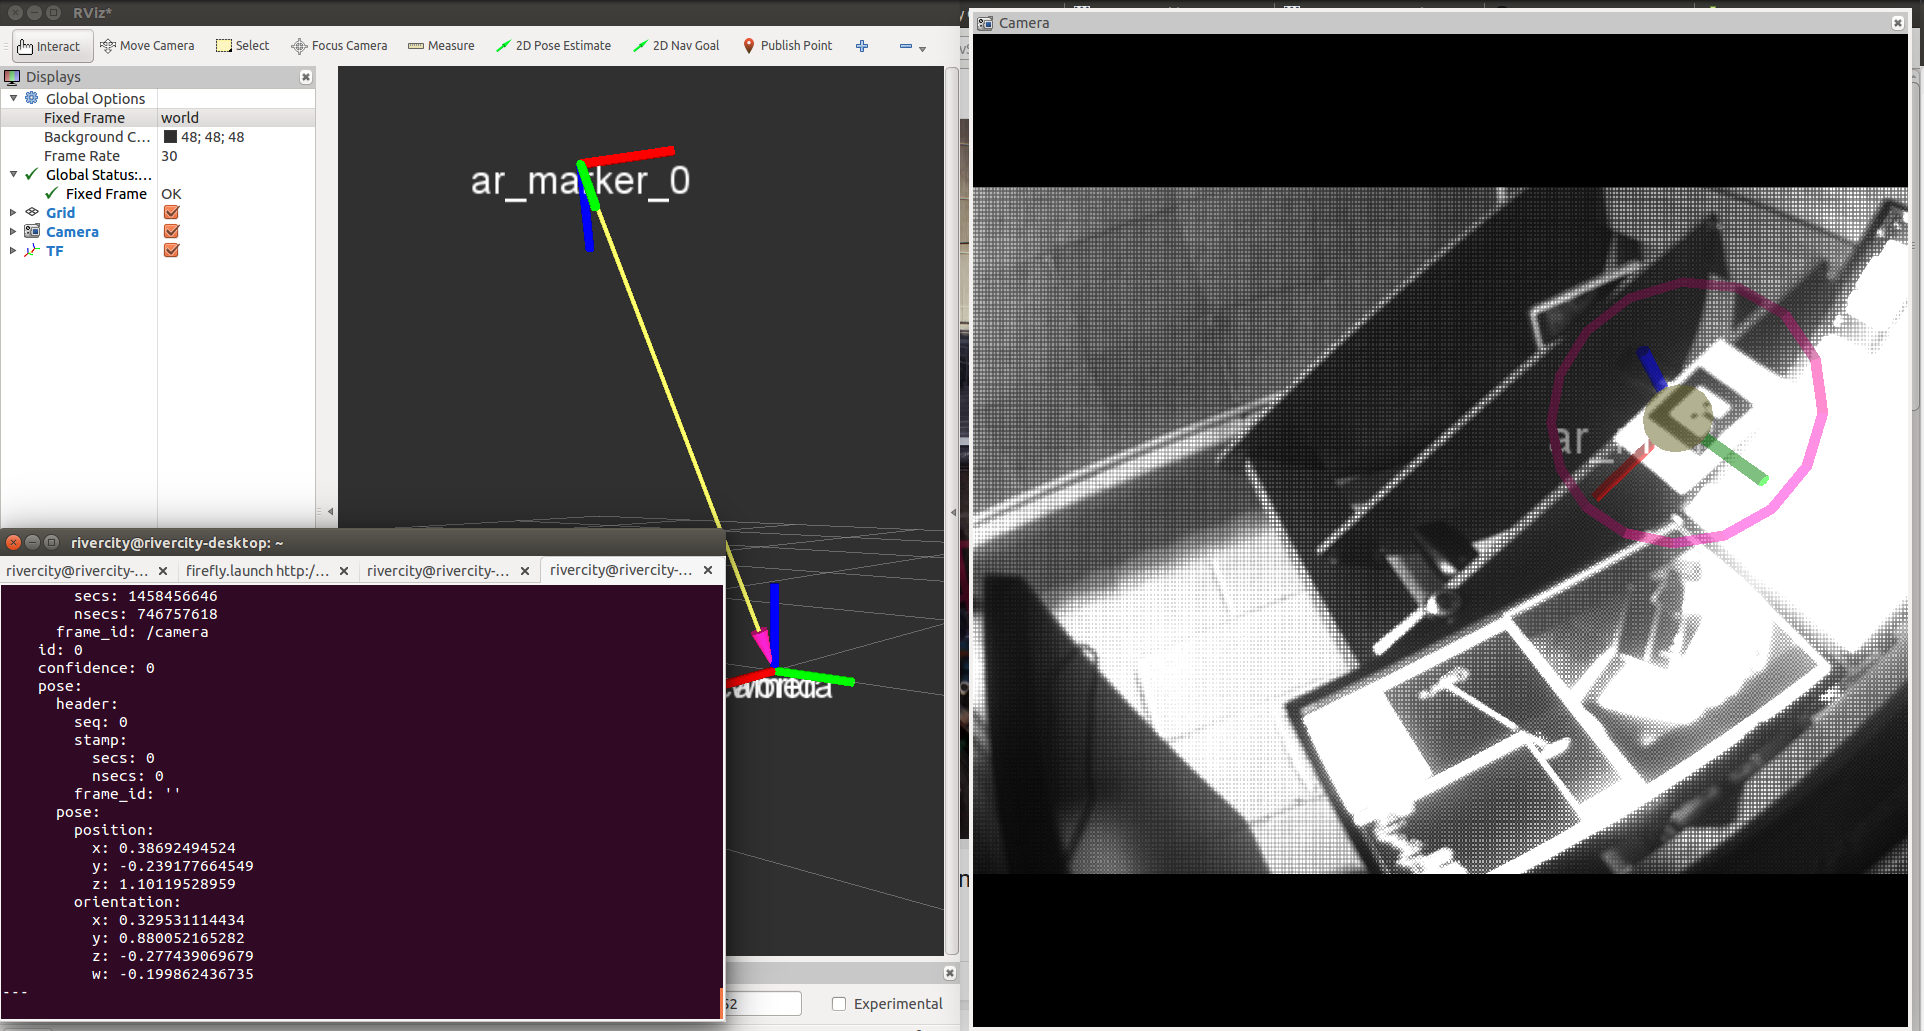
\includegraphics[width=1\textwidth]{images/alvar2.png}
\end{frame}


%% END SECTION 2



%% BEGIN SECTION 3
% How do we plan to integrate the different systems together
\begin{frame}{Testing: U-1}
\textbf{As a user, I want to communicate the waypoints to the UAV.}
\begin{tabular}{| c | >{\raggedright}m{4cm} | m{4cm} | c |}\hline
	Task No. & Task & Test\\\hline
	3 & Modify mission communication implementation as necessary & User is able to create mission file with ground control station.\\\hline
	3 & Modify mission communication implementation as necessary & User is able to load mission file on offboard(ODroid).\\\hline
	3 & Modify mission communication implementation as necessary & Landing Algorithm on offboard starts after completing last mission.\\\hline
	
\end{tabular}

\end{frame}
% How are we going to test the UAV 
\begin{frame}{Testing: O-1}
\textbf{As an owner, I want the UAV to autonomously take-off from the landing pad.}
\begin{tabular}{| c | >{\raggedright}m{4cm} | m{4cm} | c |}\hline
	Task No. & Task & Testing\\\hline
	3 & Modify/Rewrite take-off imlementation as necessary
 & FCU recieves take-off mission from mission from offboard control.\\\hline	
	3 & Modify/Rewrite take-off imlementation as necessary
 & FCU executes take-off mission.\\\hline	
\end{tabular}
\end{frame}

\begin{frame}{Testing: O-2}
\textbf{As an owner, I want the UAV to autonomously navigate through a set of waypoints.}
\begin{tabular}{| c | >{\raggedright}m{4cm} | m{4cm} | c |}\hline
	Task No. & Task & Test\\\hline
	3 & Modify/Rewrite waypoint navigation implementation as necessary & FCU receives navigation missions from offboard control.\\\hline
	3 & Modify/Rewrite waypoint navigation implementation as necessary & FCU executes navigation in sequence.\\\hline
	3 & Modify/Rewrite waypoint navigation implementation as necessary & FCU follows, reasonably, the planned navigation.\\\hline
\end{tabular}
\end{frame}
\begin{frame}{Testing: O-3}
\textbf{As an owner, I want the UAV to autonomously return to the location of the landing pad.}
\begin{tabular}{| c | >{\raggedright}m{4cm} | m{4cm} | c |}\hline
	Task No. & Task & Test\\\hline
	3 & Modify navigate to landing waypoint implementation as necessary & FCU receives last navigation mission from offboard control.\\\hline
	3 & Modify navigate to landing waypoint implementation as necessary & FCU executes navigation mission.\\\hline
	3 & Modify navigate to landing waypoint implementation as necessary & FCU navigates within a reasonable distance(\textless 10m) to waypoint.\\\hline
\end{tabular}
\end{frame}

% How are we going to test the VH Landing Algorithm
% Maybe discuss tests at the different stages (blob color recog, dist/dir output, real-time output (How many frames?)) 
\begin{frame}{Testing: O-4}
	\textbf{As an owner, I want the UAV to autonomously land on the landing pad without damaging the craft}
	\begin{tabular}{| c | >{\raggedright}m{4cm} | m{4cm} | m{4cm} |}\hline
		Task No. & Task & Test \\\hline
		4 & Modify landing pose implementation as necessary & UAV accurately estimates pose of AR tag\\\hline
		4 & Modify landing pose implementation as necessary & UAV centers over AR tag(\textless 0.1m).\\\hline
		4 & Modify landing pose implementation as necessary & The UAV remains centered during descent.\\\hline
		4 & Modify landing pose implementation as necessary & The UAV lands without damaging craft or legs.\\\hline
		
	\end{tabular}
\end{frame}
\begin{frame}{Testing: O-5}
\textbf{As an owner, I want the UAV to autonomously land on the landing pad with the correct orientation.}
\begin{tabular}{| c | >{\raggedright}m{4cm} | m{4cm} | m{4cm} |}\hline
	Task No. & Task & Test\\\hline
		4 & Modify landing orientation implementation as necessary & UAV accurately estimates the orientation of AR tag\\\hline
		4 & Modify landing orientation implementation as necessary & UAV changes orientation to align with AR tag.\\\hline
		4 & Modify landing orientation implementation as necessary & UAV maintains correct orientation during descent.\\\hline
\end{tabular}
\end{frame}

\begin{frame}{Remaining Backlog}
\begin{itemize}
\item \textbf{Owner 4(O-4)}
\item \textbf{Owner 5(O-5)}
\end{itemize}

\end{frame}


\begin{frame}{Revised Goals}
	\begin{itemize}
		\item User will need to create file containing missions for offboard control to use, not 
		\item Use of only AR Tag, not AR Tag + Landing Lights.
	\end{itemize}

\end{frame}


%% END SECTION 3

\begin{frame}{Risk Analysis}
\begin{itemize}
\item Localization: Without a better approach to localization, our estimates of our current pose are very poor. As a result our UAV is unable to navigate to the AR tag.
\end{itemize}


\end{frame}

\begin{frame}{Risk Mitigation}
\begin{itemize}
\item Localization
\begin{itemize}
\item Use visual odometry with the camera we already are using
\item Attach more sensors if necessary
\end{itemize}

\end{itemize}

\end{frame}


\begin{frame}{Timeline}
\textbf{Sprint 6 3/21/16~4/15/16}
\begin{itemize}
\item Finish Landing Algorithm Simulations(O-4,O-5)
\end{itemize}
\vspace{2mm}
Sprint 6 necessitates solving our localization issues, so that we can combine our vision and message passing framework to complete this project.
\end{frame}

\begin{frame}{Budget}
\begin{table}[]
\centering
\begin{tabular}{|l|l|l|l|}
\hline
Item               & Qty & Price    & Total    \\ \hline
                   &     &          &          \\ \hline
Frame              & 1   & \$79.99  & \$79.99  \\ \hline
Motors             & 8   & \$23.99  & \$191.92 \\ \hline
ESCs               & 8   & \$17.78  & \$142.24 \\ \hline
Pixhawk            & 1   & \$199.99 & \$199.99 \\ \hline
Power Distribution & 1   & \$19.99  & \$19.99  \\ \hline
GPS Mast           & 2   & \$10.00  & \$20.00  \\ \hline
GPS                & 2   & \$89.99  & \$179.98 \\ \hline
Power Module       & 1   & \$24.99  & \$24.99  \\ \hline
Odroid XU4         & 1   & \$75.95  & \$75.95  \\ \hline
Props(set of 4)    & 3   & \$7.55   & \$22.65  \\ \hline
                   &     &          &          \\ \hline
TOTAL              &     &          & \$957.70 \\ \hline
\end{tabular}
\end{table}


\end{frame}


\begin{frame}{IP \& Licensing}
Intellectual Property:\\
Project is owned by SDSMT\\
\vspace{2mm}
Licensing for Dependencies:
\begin{itemize}
\item OpenCV: BSD 
\item ROS: BSD
\item Mavlink: LGPL version 3
\item QGroundControl: GPL version 3
\item ROS Packages
\begin{itemize}
\item mavros: GPLv3, LGPLv3, BSD
\item svo: GPLv3 licence
\item ar\_track\_alvar: BSD
\item pointgrey\_camera\_driver: BSD
\item usb\_cam: BSD
\end{itemize} 
\end{itemize}

Additionally, all members of the team are registered with the FAA and have received their drone pilot's license.

\end{frame}

%% END SECTION 4


%% BEGIN SECTION 5
\begin{frame}{Prototypes and Demos}
\large{\textbf{Demos}}
\begin{itemize}
	\item Communication
	\item Offboard Control
	\item AR Track Alvar
\end{itemize}

\end{frame}



%% END SECTION 5
\begin{frame}{ END}
\centering	Questions
\end{frame}



\end{document}
